\section{Prospective confirmation in a new field and larger model}\label{sec:fresh}
The frozen new-world protocol was completed without inspecting any compound score during fitting. Seventeen independently sampled corpora, supports, validation sets, test sets and source initializations in $\F_{17}$ replace the shared old-world data. Each test contains 2,000 collision pairs and 512 IID inputs. The hidden width is 512 instead of 128. The joint encoder/generator preparation minibatch index stream retains the shared legacy scheduling code; data, model initialization and first/second-operator fitting streams vary. Randomly sampled units can overlap across units, but no weights are reused. This is one new algebraic system with independent random datasets, rather than 17 distinct systems.

\paragraph{Fixed design and two primary tests.}
Correct versus answer-matched incorrect first-step correspondence is crossed with the same parameter-matched Identity/GELU predictor. Correct output distillation, inputs, steps and encoder are identical within a unit. All 68 first predictors and 51 second-step noise candidates were fit before the test was opened. Second-step noise is chosen only by known single-step validation and is shared across the first-predictor arms. No compound label or compound target state enters training. The two predeclared source-level contrasts use paired two-sided $t$ tests with Holm correction; reported 95\% intervals are marginal rather than simultaneous.

GELU correct minus incorrect compound accuracy is 5.157 pp, with interval [1.924,8.391] pp and Holm $p=0.00381$. Natural null versus row interchange donor-target accuracy is 49.322 pp, with interval [43.527,55.117] pp and Holm $p=9.3\times10^{-12}$. Row interchange is a localization diagnostic that can change first logits; null interchange preserves them. All 17 units are retained.

\begin{table}[ht]\centering\small
\begin{tabular}{lrrrr}\toprule First predictor & Compound (\%) & Both (\%) & First (\%) & State MSE\\\midrule
linear correct & 6.75 & 0.34 & 99.96 & 0.1431 \\
linear wrong & 6.11 & 0.24 & 99.96 & 0.1968 \\
nonlinear correct & 11.52 & 1.52 & 99.95 & 0.0699 \\
nonlinear wrong & 6.36 & 0.27 & 99.96 & 0.2087 \\
\bottomrule\end{tabular}
\caption{Mean collision performance with the validation-selected second operator in the new field. Datasets and initializations both vary across the 17 statistical units.}
\end{table}

\paragraph{Error decomposition and the performance gate.}
The selected second operator reaches 99.73\% on true intermediate states, versus 11.52\% with correctly paired GELU predictions. The mean fraction of the oracle--incorrect gap closed is 5.53\%. This contrasts first-state error with downstream failure and does not treat first-answer accuracy as state sufficiency. The original second operator, all IID results and all individual units are also archived. The preregistered 40\% performance gate is not passed. No further candidate was selected by compound results.

\paragraph{Natural-state interchange and its invalidation control.}
Donors have the same first gold answer, lie in a different orbit and are used once per arm. Distinct-future null donors are followed in 52.02\%, compared with 2.70\% for distinct-future row donors. Same-future null donors retain the donor answer in 71.93\%, but change 28.10\% of predictions; the preregistered 5\% change gate is not passed. The maximum first-logit change for null interchange is $1.98\times10^{-13}$. Even natural components can yield off-manifold hybrids. These findings concern downstream answer-information transport, not identification of natural mathematics-specific relation coding.

\paragraph{Scope and equivalence.}
The larger model, increased input coverage, new field and noisy second-step fitting change together. This confirmation cannot isolate a width effect. It also does not fit the converged affine baseline in the new world; any finite-budget activation contrast is not a convergence or equivalence result. The old affine--GELU TOST analyses remain secondary and posthoc, with the primary wording ``additional advantage was not confirmed'' limited to the old unregularized diagnostic. Independent replay reconstructs 2,161,059 label, split, prediction and invariant entries; it validates the registered computation without strengthening its causal scope.

\begin{figure}[ht]\centering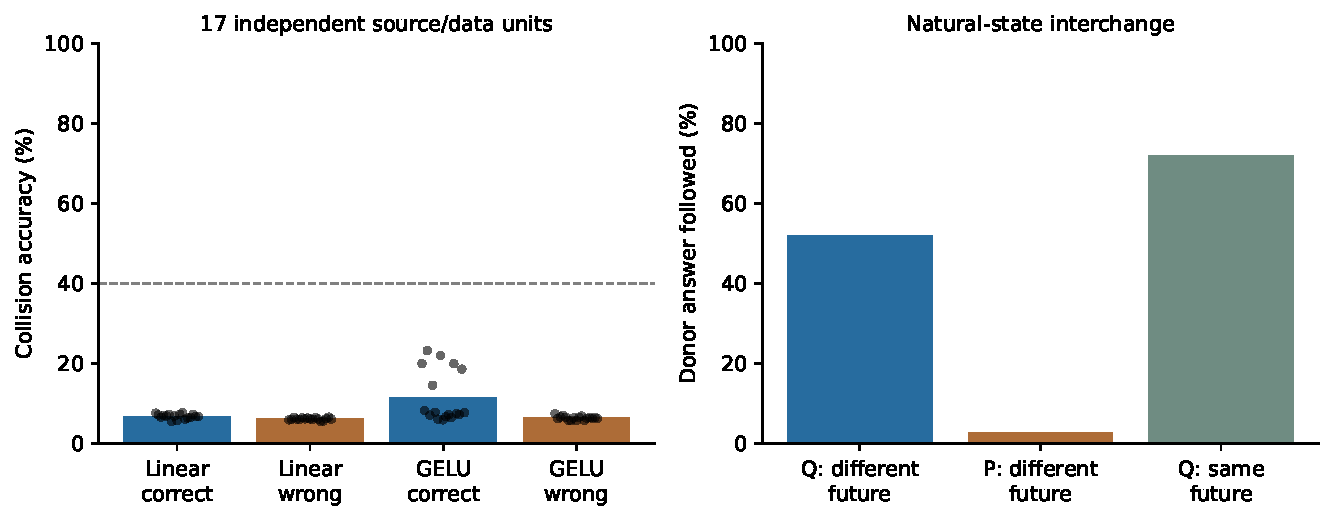
\includegraphics[width=\linewidth]{figures/reviewer_fresh.pdf}
\caption{Frozen new-field confirmation. Points are independent source/data units; the dashed line is the predeclared 40\% accuracy gate. Natural-state swaps address downstream information transport.}
\end{figure}
